This section provides a brief description of features of MedTech. The primary operational aspects is it to assist medical professionals with the health care of patients. MedTech aims to increase efficiency and usability of EMR systems. This section provides the reader with an overview of our EMR System, MedTech. Below we outline the key features and functions found in the products as well as critical user interactions and user interfaces from the perspective of end users, maintainers and administrators. 

\subsection{Features \& Functions}

The main features we hope to target are: 

1) Hourly updates from patient to health care professionals 

2) Voice recognition verification from doctors to patients for medications, prescriptions 

3) Patient history details like previous ailments, medications, prescriptions, allergies and others. 

4) Integration of machine learning and other deep learning models to help with early diagnosis 

5) Updating lab results and other diagnostics in to the software 

6) Conversion of notes from medical professionals to billing and other document management. 

Since the medical field is a diverse industry and includes a variety of specializations, we will be focusing on a select department so as to narrow down our focus. 





\section{Sprint Backlog}
External inputs and outputs are outlined in the table below:  \\ % work units do not have to be hours, change text accordingly


\begin{tabular}{| p{1in} | >{\centering\arraybackslash} p{2in} | >{\centering\arraybackslash} p{2in} |}
\hline
NAME & DESCRIPTION & USE \\ \hline
Login & A login page for medical professionals & To login with their credentials  \\ \hline
Patient File Summary & Brief description of patient's file & This would display patient basic information, allergies, ID and blood type \\ \hline
Patient Updates & Updates by doctors,pharmacy and other health care professionals  & This would include updates to treatment plan,pharmacy prescriptions and other orders from doctors \\ \hline
Settings & This would be to help with UI/basic web settings & Provide users with options to change password and other basic operations \\ \hline
Logout & A button to exit  & This will logout out of professional's particular page. \\ \hline
Other elements & elements pertaining to individual patients & It would include patient for lab,flowsheet, patient history and updates all would appear on the same page \\ \hline

\end{tabular}
\pagebreak

\subsection{Product Interfaces}
Below we have mock ups for our login page and patient file summary. 

\begin{figure}[h!]
	\centering
   	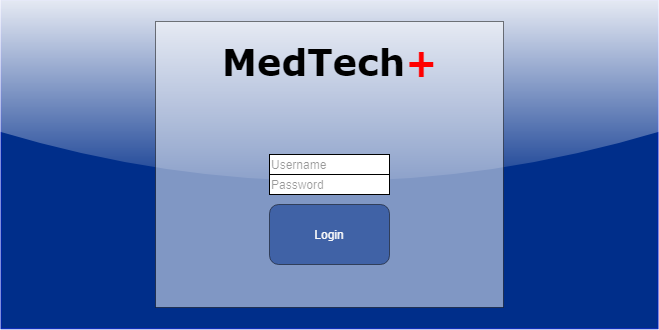
\includegraphics[width=1.00\textwidth]{images/Login.png}
    \caption{Login}
\end{figure}

\begin{figure}[h!]
	\centering
   	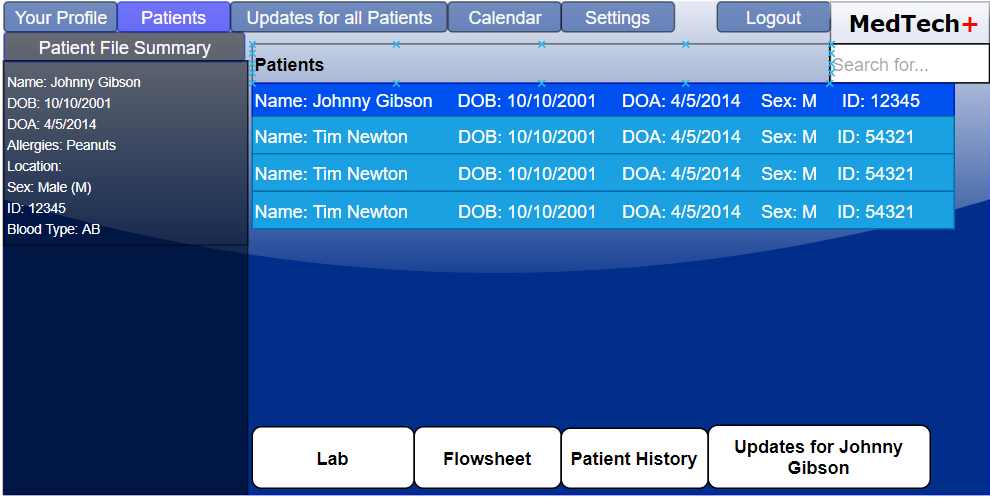
\includegraphics[width=1.00\textwidth]{images/afterlogin.PNG}
    \caption{After Login}
\end{figure}